\chapter{Methods}
\label{cha:methods}

The goal in this work was to develop a CNN architecture that is able to predict surgical instrument segmentation and location in endoscopic images. All networks are evaluated on EndoVis15 (see section~\ref{sec:endovis15}) and EndoVis17-S (see section~\ref{sec:endovis17}) datasets.
When two instruments are visible at the same time in the input video frame, they are not distinguished by the network. This is done in a postprocessing step.

The approach in this work is to use the information learned by a CNN for instrument segmentation to improve the instrument localization task. When transforming the localization ground truth to the same shape as the segmentation ground truth (see section~\ref{sec:heatmaps}), both tasks can share the parameters of the CNN. This seems to be an advantage in comparison to other localization approaches, as showed recently by Laina et al.~\cite{Laina2017}.
  
\section{Instrument Segmentation Network}
\label{sec:TernausNet_11}
In this work, TernausNet-11 is chosen as basis segmentation network and then extended to solve the localization task.
TernausNet-11 (see figure~\ref{img:ternausnet_11}) is proposed in the winning paper of EndoVis17-S by Shvets et al.~\cite{Shvets2018}. 
The encoder part is a VGG11-Network~\cite{simonyan2014vgg} pretrained on ImageNet~\cite{imageNetWinner2012krizhevsky}. Every convolutional layer of the network is followed by a ReLU activation function. 

The output of TernausNet-11 is a binary image, that contains a white segmentation mask where the instrument is located (see figure~\ref{img:model01_dataset2_good_pred}).

\begin{figure}
\centering
\begin{subfigure}[t]{0.49\textwidth}
	\centering
	\includegraphics[width=0.65\textwidth]{images/predictions/model01/orig_Dataset2_frame006.jpg}
	\caption{Example input image.}
	\label{img:model01_dataset2_input_image}
\end{subfigure}
\begin{subfigure}[t]{0.49\textwidth}
	\centering
	\includegraphics[width=0.65\textwidth]{images/predictions/model01/Dataset2_model01_frame006_mask.jpg}
	\caption{Predicted instrument segmentation frame by TernausNet-11.}
	\label{img:model01_dataset2_good_pred}
\end{subfigure}
\caption[Example EndoVis15-S prediction]{Example input image out of EndoVis15-S with corresponding predicted mask by TernausNet-11.}
\label{img:example_segm_pred+gt_unet11}
\end{figure}

As TernausNet-11 outperforms the other networks for the different segmentation challenges except TernausNet-16, which has a larger inference time, TernausNet-11 is chosen as basis for the Localization Network (see section~\ref{sec:tracking_net}).
 
%To solve this task, the segmentation network TernausNet-11~(see section~\ref{sec:TernausNet_11}) is adjusted: It is extended to predict both segmentation and localization of the surgical instruments~(see section~\ref{sec:tracking_net}).

\begin{figure}
	\centering
	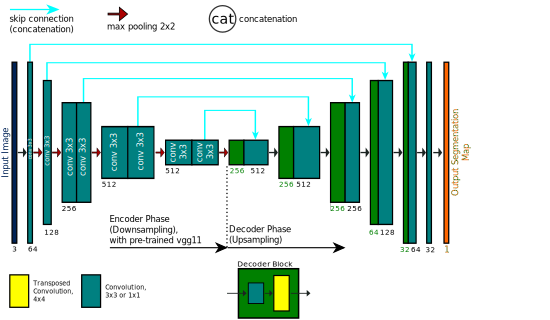
\includegraphics[width=.9\textwidth]{images/networks/TernausNet11_description.png}
	\caption[Structure of TernausNet-11]{Structure of TernausNet-11. The network is proposed by Shvets et al.~\cite{Shvets2018}. 
The blue boxes represent feature maps, the number of channels is denoted below each box. In the decoder phase of the network, each green box is a decoder block that consists of a convolution followed by a transposed convolution. 
The blue arrows denote skip connections:
The feature maps from the encoder phase are concatenated to the decoder blocks in the upsampling phase of the network. 
The red arrows represent 2x2 max pooling operations. The orange box represents the segmentation output of the network.
	}
	\label{img:ternausnet_11}
\end{figure}

TernausNet-11 is trained for the image segmentation task using the loss function $L_{segm}(y_{w,b}(x_j),t_j)$. It consists of two parts:

\begin{equation}
\label{eq:loss_segmentation}
L_{segm}(y_{w,b}(x_j),t_j) = BCE(y_{w,b}(x_j),t_j) - \log J_{binary}(y_{w,b}(x_j),t_j)
\end{equation}

%The first part is the \emph{binary cross entropy (BCE)} loss~(see equation~\ref{eq:bin_crossentropy}), that is combined with a sigmoid function: $BCE_{sigm}$~(see equation~\ref{eq:sigmoid_bin_crossentropy}). 
The first part is a binary cross entropy loss (BCE) combined with a sigmoid function:

\begin{equation}
\label{eq:sigmoid_bin_crossentropy}
BCE_{sigm}(y_{w,b}(x_j),t_j) = -\frac{1}{N}\sum_{i=1}^N{[t_j \log(\sigma(y_{w,b}(x_j)))+(1-t_j)\log(1-\sigma(y_{w,b}(x_j))]}
\end{equation}

Combining the sigmoid function with the BCE loss - instead of applying the sigmoid function first and BCE in a second step - increases the numerical stability.~\cite{murphy2006naive}

The second part of $L_{segm}(y_{w,b}(x_j),t_j)$ is a Jaccard loss for binary evaluation:

\begin{equation} \label{eq:loss_jaccard}
J_{binary}(y_{w,b}(x_j),t_j) = \frac{1}{N} \sum_{i=1}^N \frac{t_j \cdot y_{w,b}(x_j)}{t_j + y_{w,b}(x_j) - t_j \cdot y_{w,b}(x_j)}
\end{equation}

$J_{binary}$ is a differentiable generalization of the Jaccard index that is adjusted to fit into the loss function of the network. It is a differentiable function and therefore suitable for using it for optimizing the network with gradient descent.~\cite{iglovikov2017satellite}

%The Jaccard index~$J(X, Y)$ (see equation~\ref{eq:general_jaccard}) The Jaccard index is taken to measure the similarity of two datasets $X$ and $Y$.

%\begin{equation}
%\label{eq:general_jaccard}
%\begin{aligned}
%J(X, Y) = \frac{\mid X \cap Y \mid }{\mid X \cup Y \mid} &= \frac{\mid X \cap Y \mid}{\mid X \mid + \mid Y \mid - \mid X \cap Y \mid} \\ \\
%0 \le & J(X, Y) \le 1
%\end{aligned}
%\end{equation}

%$J(X, Y)$ is not differentiable and therefore not suitable for using it for optimizing the network with gradient descent. % maybe ref to background  
% 
%
%\begin{equation}
%\label{eq:bin_crossentropy}
%BCE(y_{w,b}(x_j),t_j) = -\frac{1}{N}\sum_{i=1}^N{[t_j \log(y_{w,b}(x_j))+(1-t_j)\log(1-y_{w,b}(x_j))]}
%\end{equation}

\section{Instrument Localization Network}
\label{sec:tracking_net}
The network architecture that is used for localization of surgical instruments in this work is a modified TernausNet-11 (see figure~\ref{img:tracking_network_unet11based}). It is extended by three more layers: One branching layer with 32 channels, one concatenation layer where the segmentation output and the branching layer are concatenated, and one output layer for localization of the instruments.
This architecture is inspired by Laina et al.~\cite{Laina2017}.
The network predicts greyscale images, therefore the segmentation output layer and the localization output layer each have one channel.
The Localization Network is abbreviated as \emph{LocNet}.

The output of the segmentation output layer is the same as the output of TernausNet-11.
The output for the localization task is a greyscale heatmap (see section~\ref{sec:heatmaps}).
A high pixel value at the predicted heatmap indicates a high probability that the instrument center point is located at this pixel position.

\begin{figure}
	\centering
	\includegraphics[width=.8\textwidth]{images/networks/TrackingNet_description.png}
	\caption[Structure of Localization Network]{Network architecture that is used for segmentation and localization of the surgical instruments in this work. It is an extended TernausNet-11. The orange box represents the segmentation output, the grey box the localization output of the network.} 
	\label{img:tracking_network_unet11based}
\end{figure}

The output of LocNet is calculated with given input $x_j$ as a tuple $(y_{w,b}(x_j), z_{w,b}(x_j))$, where $y_{w,b}(x_j)$ is the output of the segmentation layer and $z_{w,b}(x_j)$ is the output of the localization layer.
Given the target $s_j$ as ground truth for segmentation and $t_j$ as ground truth for the localization heatmap, a combined loss for concurrent instrument segmentation and localization is defined as follows:

\begin{equation}
\label{eq:track_loss}
L_{loc}(y_{w,b}(x_j), z_{w,b}(x_j), s_j, t_j) := (1-\gamma)L_{segm}(y_{w,b}(x_j), s_j) + \gamma MSE(z_{w,b}(x_j), t_j)
\end{equation}

The segmentation loss is calculated by $L_{segm}(y_{w,b}(x_j), s_j)$, the localization loss is calculated by $MSE(z_{w,b}(x_j), t_j)$. One training sample for segmentation is denoted as $(x_j, s_j)$, one training sample for localization as $(x_j, t_j)$.
The impact of each loss on the overall loss is scaled by the factor $\gamma$.

\section{Heatmaps}
\label{sec:heatmaps}
%gauss function: cite it, explain parameters
It is necessary to convert the localization targets, given 2D image positions for EndoVis15-T, into greyscale images, in order to make it possible for the LocNet to process them.
Out of each localization target one heatmap is created.
The \emph{heatmap} is a greyscale image that has higher pixel values around the center point position of the surgical instrument (see section~\ref{sec:data_preprocessing}).

The heatmaps are generated by calculating a two-dimensional Gaussian distribution $gauss2D(x_r,y_r)$, centered at the center point $(x_{cp}, y_{cp})$ of the instrument.

\begin{equation}
\label{eq:gauss2D_function}
H(x_r,y_r)=gauss2D(x_r,y_r) = \frac{1}{\sqrt{2\pi\sigma^2} } e^{ -\frac{(x_r-x_{cp})^2 + (y_r-y_{cp})^2}{2\sigma^2} }
\end{equation}

The standard deviation $\sigma$ controls the spread of the Gaussian around the instrument location $(x_{cp}, y_{cp})$. $\sigma^2$ denotes the variance. For better interpretability, the pixel values are scaled to the range $[0, 1]$ before given to the network for training.

By iterating over the dimensions of the training input image and applying $gauss2D(x_r,y_r)$, a heatmap with the same dimensions is generated out of the ground truth instrument position.
$(x_r, y_r)$ is one pixel position of the training image, which corresponds to the pixel position in the generated heatmap.


When two instruments are visible in the input image, the heatmap is generated by calculating two Gaussian distributions, one for each instrument (see figure~\ref{img:heatmap_only_2instr}).

\begin{figure}
\centering
\begin{subfigure}[t]{0.49\textwidth}
	\centering
	\includegraphics[width=.65\textwidth]{images/dataset/robotic15_segm/heatmap_frame001-1instrument.jpg}
	\caption{Example heatmap generated from the ground truth position of one instrument.}
	\label{img:bla}
\end{subfigure}
\begin{subfigure}[t]{0.49\textwidth}
	\centering
	\includegraphics[width=.65\textwidth]{images/dataset/robotic15_segm/heatmap_frame001_2instruments.jpg}
	\caption{Example of a heatmap frame generated for the case of two visible instruments in the corresponding input image.}
	\label{img:heatmap_only_2instr}
\end{subfigure}
\caption[Example heatmap frames]{Example heatmaps generated out of the ground truth for EndoVis15-T.}
\label{img:two_heatmap_frames}
\end{figure}


\section{Postprocessing}
%%%%%% postprocessing%%%%%%
The heatmaps predicted by the network are mostly having a pixel range from $[127,255]$.
In order to improve the extraction of the instrument position, the pixel values of the predicted heatmaps are thresholded with $threshold$ set to 129 (see figure~\ref{img:thresh_pred_loc_model01}): 

\[
    thresh(H(x_r,y_r))= 
\begin{cases}
    H(x_r,y_r)& \text{if } H(x_r,y_r)\geq threshold\\
    0         & \text{otherwise}
\end{cases}
\]

In a second postprocessing step, histogram equalization~\cite{equalization_histogram1987pizer} is used to increase the contrast of the Gaussian distribution in the image (see figure~\ref{img:histogr_pred_loc_model01}).

\begin{figure}
\centering
\begin{subfigure}[t]{0.49\textwidth}
\centering
\includegraphics[width=.65\textwidth]{images/predictions/model1/thresholded-frame001-Dataset2/orig_prediction_frame001.jpg}
\caption{Unmodified localization prediction of LocNet.}
\label{img:pred_loc_model01_unmod}
\end{subfigure}
\begin{subfigure}[t]{0.49\textwidth}
\centering
\includegraphics[width=.65\textwidth]{images/predictions/model1/thresholded-frame001-Dataset2/ONLY_THRESHOLDE_Dataset2.jpg}
\caption{Thresholded localization prediction of LocNet.}
\label{img:thresh_pred_loc_model01}
\end{subfigure}

\begin{subfigure}[t]{0.49\textwidth}
\centering
\includegraphics[width=.65\textwidth]{images/predictions/model1/thresholded-frame001-Dataset2/THRESHOLD_and_equalized_Dataset2.jpg}
\caption{Equalized localization prediction of LocNet in order to increase contrast.}
\label{img:histogr_pred_loc_model01}
\end{subfigure}
\begin{subfigure}[t]{0.49\textwidth}
\centering
\includegraphics[width=.65\textwidth]{images/predictions/model1/thresholded-frame001-Dataset2/superimposed_preproc_heatmap_frame001.png}
\caption{Input frame out of EndoVis-15 with superimposed postprocessed heatmap.}
\label{img:superimposed_heatmap_thresh_model01}
\end{subfigure}
\caption[Postprocessing steps predicted heatmap]{Example sequence for postprocessing a predicted heatmap. First, the original heatmap (a) is thresholded (b). Afterwards, the contrast is increased by histogram equalization (c). Figure (d) shows the postprocessed heatmap with underlying corresponding input image}
\label{img:threshold_steps}
\end{figure}

%%%%%%% K-MEANS %%%%%%%%%%%%%%
To get the instrument position out of the thresholded heatmap, \emph{k-means} clustering is used. It is a commonly used method to automatically partition a dataset into $k$ groups.~\cite{k-means-paper2005sipkins}
When the input to the corresponding predicted heatmap contains one instrument, $k$ is set to 1. When two instruments are visible in the input image, $k$ is set to 2.
The pixel values of the thresholded heatmap are used as weights for the k-means clustering to improve the results, because a higher pixel value indicates a higher probability that the instrument center is located at that position.

\section{Evaluation Metrics}
\label{sec:evaluation_metrics}
% sources -> already have 2 papers
The following section gives an overview of the evaluation metrics that are commonly used for the validation of NNs. As the network in this work is used for binary classification, the evaluation methods proposed in this section cover only the evaluation of predictions with two classes. The descriptions are adjusted for evaluating LocNet.
There are two classes for binary classification: \emph{Positive} if a pixel in an input image is part of a surgical instrument and \emph{negative} if the pixel belongs to the background. The prediction of a model for one pixel is evaluated as \emph{true} if the predicted class is correct, or \emph{false} if it is wrong. 

Each output predicted by a model can be classified in one of four categories: 

\begin{itemize}
\item $TP\:(true\:positive)$ \\
Represents the number of pixels correctly labeled as surgical instrument.
\item $TN\:(true\:negative)$ \\
Represents the number of pixels correctly labeled as background.
\item $FP\:(false\:positive)$ \\
Represents the number of pixels which are erroneously labeled as surgical instrument but actually are part of the background.
\item $FN\:(false\:negative)$ \\
Represents the number of pixels which are erroneously labeled as background but actually are part of a surgical instrument in the image.
\end{itemize}

The \emph{precision} evaluates the proportion of predicted positive classes ($TP+FP$) that are actually positive classes ($TP$).

\begin{equation}
\label{eq:precision}
\text{precision}=\frac{TP}{TP+FP} 
\end{equation}

The evaluation metric \emph{recall} (see equation~\ref{eq:recall}), in literature also denoted as \emph{sensitivity}, \emph{hit rate} or \emph{true positive rate}, is the proportion of actual positive classes ($TP+FN$) that are correctly predicted as positive ($TP$).~\cite{powers2011eva_recall_precision}
% the amount of all pixels that correspond actually to a surgical instrument - pixels that are correctly identified as instrument ))

\begin{equation}
\label{eq:recall}
\text{recall}=\frac{TP}{TP+FN}
\end{equation}

The evaluation metric \emph{specificity}, also called \emph{true negative rate}, measures the proportion of all pixels that correspond to the negative class ($TN+FP$) that are correctly identified as this class ($TN$).
It can be seen as inverse recall because it works the same way as the recall metric, but takes into account the negative examples instead.~\cite{powers2011eva_recall_precision}

\begin{equation}
\label{eq:specificity}
\text{specificity}=\frac{TN}{TN+FP}
\end{equation}

The evaluation metrics precision and recall focus only on the positive examples and predictions. Neither of them captures information about how the model is handling negative cases.~\cite{powers2011eva_recall_precision}
\emph{Intersection over Union~(IoU)}, also referred to as \emph{Jaccard index}, can be seen as a combination of these two metrics.
It is considered as a better segmentation metric for evaluating binary images because it penalizes both over- and undersegmentation.~\cite{Attia2017_surg_tool_cnn-rnn}
% penalizing oversegm: precision, penalizing under segm: recall

\begin{equation}
\label{eq:iou}
\text{IoU}=\frac{TP}{TP+FP+FN}
\end{equation}

\emph{Dice} (see equation~\ref{eq:dice_binary}) measures the overlap between two binary images~\cite{dice_eva2008babalola}. It is similar to $IoU$, which counts $TP$ only one time in both the numerator and denominator.

\begin{equation}
\label{eq:dice_binary}
\text{dice} = \frac{2 TP}{2 TP + FP + FN}
\end{equation}

\emph{Accuracy} is the proportion of all correct predictions~($TP+TN$) among the total number of cases~($TP+TN+FP+FN$).
The advantage over recall, precision, and $IoU$ is that accuracy explicitly takes into account the classification of negative cases~\cite{powers2011eva_recall_precision}.

\begin{equation}
\label{eq:accuracy}
\text{accuracy}=\frac{TP+TN}{TP+TN+FP+FN}
\end{equation}

The appropriateness of evaluating a model with the accuracy metric depends on the distribution of the dataset. High accuracy results can depend on the distribution of the dataset: Assumed in a surgical instrument dataset the instrument is very small or there are many sequences where no instrument is visible, a model that always predicts the negative case that only background is visible, will achieve high accuracy because the $FN$ rate will be very low.~\cite{metz1987accuracyROC}
% FN rate: erroneously pixels classfied as background but actually belonging to a surgical instrument
% all pixels correctly classified as instrument and background - all pixels in the image
Using \emph{balanced accuracy (b.acc.)} for the evaluation decreases this dependency on the dataset.~\cite{balanced_accuracy2010brodersen}

\begin{equation}
\label{eq:balanced_accuracy}
\text{balanced accuracy}=\frac{1}{2}\left(\frac{TP}{TP+FN}+\frac{TN}{TN+FP}\right)
\end{equation}



